\hypertarget{position-velocity-and-orientation-sensors}{%
\section{Position, Velocity and Orientation
Sensors}\label{position-velocity-and-orientation-sensors}}

Navigation and localization is one of the more challenging problems in
mobile robotics and any estimate is welcome. If you have an estimate on
wheel velocity then you can by integration estimate rotation and through
wheel diameter estimate the linear travel (over very short distances).
Using the differential drive equations, \texttt{ddkinematicsmodel}, the
wheel velocity may be integrated to determine position in the global or
inertial reference frame. So the obvious question is... how do we
determine wheel position or velocity?

\texttt{Position\ sensors} measure the absolute displacement of a joint
or other sensed item for both linear and rotary joints. Both analog and
digital technologies are used for measuring displacement. Variable
resistors have been common for years. Either as a rotary device such as
found in volume dials or slider (fader) such as found in mixers. The
rotary variable resistor is known as a potentiometer or "pot" for short.
Typically wired in a voltage divider (discussed later), the voltage
across the potentiometer can be measured as an analog signal. It can be
converted to a digital signal for use in a microcontroller. Variable
resistors have an element which slides over a coil of resistive wire or
over carbon base changing the electrical path which varies the
resistance.

A direct digital approach is to use \texttt{encoders}. Absolute encoders
return a Gray code as a function of position. These also come in linear
and rotary designs. Typically one has a collection of sensors which can
detect light and dark. The encoder allows light to pass through it in
some pattern that correlates to position. The sensed pattern is
converted to the output code. Another approach used is to count the
number of times a particular pattern occurs or a beam is interrupted.
This is explored in detail below with the optical wheel encoders which
can be used for velocity in addition to position estimates.

\begin{quote}
Position sensors: (a) Potentiometer, (b) Fader, (c) Encoder.
\end{quote}

\hypertarget{tachometers}{%
\subsection{Tachometers}\label{tachometers}}

An electric motor and a generator are very similar devices which just
operate in opposite fashions. Providing electrical power in a motor
causes the shaft to turn. Conversely turning the shaft of a generator
produces electricity. A \texttt{tachometer} can be built out of a
generator (or electric motor). The faster the shaft spins, the greater
the voltage or higher the frequency produced. This can be converted to a
digital signal and thus provides a measure of rpm.

\hypertarget{optical-wheel-encoders}{%
\subsection{Optical Wheel Encoders}\label{optical-wheel-encoders}}

One option to tackle measurement of rotation is known as an optical
wheel encoder. We will discuss two common types, the incremental and
absolute encoders. They operate by focusing a beammof light onto a
pattern mounting to the rotating surface. That pattern is read and the
rotation or rotation increment is computed. The dominant lighting source
in electronics and robotics, are \texttt{Light\ Emitting\ Diodes}, or
LEDs\footnote{LEDs have a variety of operating specs and you have to
  read the datasheet to find out about the specific voltage-current
  properties. Normally one is given an operating range and one must work
  out a suitable way to power the diode. For example, assume we have and
  LED which operates in the 3-6 volt range and targeted current level is
  20mA. If we select \$V = 5\$, then the resistor should be \$R = V/I =
  5/.02 = 250\$. Since 250 is not a standard value, we select the
  closest available resistor value which is \$R =270\$ ohms.} which can
run on very low power, are available in many frequencies and can switch
on/off quickly. \texttt{circuitled}.

\begin{quote}
LED
\end{quote}

LEDs can emit in non-visible ranges, ultraviolet and infrared. Many of
the non-visible frequencies are popular for simple object detection in
combination with a phototransistor, \texttt{IRobstacleLED}. In this
example, the infrared LED shines on some object and is reflected back to
the phototransistor. The IR light activates the transistor and causes it
to switch on and pull the output to low.

\begin{quote}
Infrared LEDs used for obstacle detection.
\end{quote}

This system can be used for simple occupancy detection or close obstacle
detection. We can also use the LED-transistor combination to determine
wheel rotation; to measure the speed or position of a wheel or dial. For
example the dials on electronic devices like a volume control. In
addition, knowing wheel rotation can assist in the process of localizing
the robot. The fundamental idea is to generate a radial or linear
pattern of black and white stripes (or slits). The IR light is either
reflected or not. This is sensed with the phototransistor. Counting the
stripes (or lists) can provide an estimate of wheel rotation. Over a
fixed interval of time this provides an estimate of wheel velocity. The
estimate is clearly improved if more stripes (or slits) per revolution
are used.

\begin{quote}
Mounting for the encoder sensor
\end{quote}

There are two basic components needed to build your own
\texttt{incremental\ encoder}. First you need the light source and the
detector. Second you need a pattern. To read the pattern, you will need
an optical sensor. Typically one uses an IR LED (IR light emitting
diode) and phototransistor pair, \texttt{ledopticalsensor}. These are
packaged in single units, for example the Fairchild QRD1313. This has
the LED and the phototransistor packaged into a unit that is 6.1mm x
4.39mm x 4.65mm (height).

\begin{quote}
IR LED (IR light emitting diode) and phototransistor pair.
\end{quote}

An encoder pattern may simply be a pattern printed on paper and attached
(glued) to the inside of a robot wheel. Simple encoder patterns are just
alternating black and white radial stripes. Two examples are given in
\texttt{encoderpattern}.

\begin{quote}
Wheel encoder pattern (a) with 1-1 ratio, (b) with 1-4 ratio.
\end{quote}

This encoder pattern will generate in idea conditions a square wave if
one continuously samples the state of the phototransistor. See
\texttt{squarewave}. Our system is digital and we don't use the raw
voltage signal. That signal is sampled by some type of analog to digital
hardware. For example, the output of the phototransistor is connected to
a general purpose I/O line (GPIO) on a microcontroller. The
microcontroller input will threshold the signal. Anything below a
certain voltage will be considered \emph{low} or zero volts. Above a
threshold voltage level it will be considered \emph{high} or max voltage
for the input. The low or high on the line is then the 0 or 1 when the
value is read in the code.

\begin{quote}
A square wave generated by the phototransistor sensing the rotating
pattern.
\end{quote}

In reality the wave will not be square. The light source and the
sensitivity of the detector as well as the thresholding might trigger
high for much greater percentage of the time. Sometimes their is
sufficient light that the system never pulls low (or the opposite). This
is the reason you may need to use the pattern shown in
\texttt{squarewave} (b). Hooking the output of the sensor to a
oscilloscope can give you an idea of the wave shape. {[}You will need to
run the motor and encoder. Mount them, hook a power supply and then hook
to the oscilloscope. If youn have a clean square wave - great.{]}

There are two common ways that reading the GPIO input can be done. One
is known as \texttt{polling} and the other as \texttt{interrupts}.
\emph{Polling} requires that the hardware samples the sensor (the GPIO)
at a regular rate. In simple applications this is done just by putting
the GPIO read in a loop. The loop is not always uniform when it reads,
but it can be good enough for some applications.

The digital signal is then converted to a binary stream as seen in
\texttt{squarewave\_sample}. When the rotation speed increases, then the
number of zeros or ones in the uniform part of the sequence will
decrease. By counting, one can gain an estimate of the square wave
period and then of rotational velocity. Unless you know that the square
wave will always have 50\% duty cycle, you should start and end counting
at the transition from 0 to 1. The period can be computed from
\(T = n \Delta t\), where \(n\) is the previous count.

Assume that you have \(k\) bands (black or white, not both) and the
period was measured to be \(T\). The rotational velocity (radians) is

\[\omega = \frac{2\pi}{kT}\]

Since there is finite time between samples, there is an error in the
estimate of the rotational velocity. The problem is that you don't know
exactly when the transition from low to high or high to low occurred.
This will introduce some measurement error. This error is higher for
systems with fewer bands (wider bands) or slower rotational velocities.

\begin{quote}
Using polling to sample the square wave.
\end{quote}

If we want to get a more accurate sense of the period of the square
wave, then we need to implement interrupts. You need hardware that
supports interrupts on a GPIO input. \emph{Interrupts} cause a change in
the program flow. WHen an interrupt occurs, the current program is
suspended and the execution jumps to special code, the interrupt
handler. This handler does the necessary work to deal with the situation
and then the system returns to the program.

In this case, we set the GPIO to generate an interrupt when the line
goes from low to high. This gives us the front edge of the square wave.
The interrupt handler can grab the current time and store it in a global
variable. It will compute the difference between the current interrupt
time and the last one. It can store the period in a global variable as
well. The global variable is available to other programs that would like
to know the period from which the rotational velocity is estimated.

\begin{quote}
Using interrupts to determine the period and thus the rotational
velocity.
\end{quote}

Although the interrupt approach is more complicated to program, it
provides more accurate timings. However, updates only occur when the
interrupt occurs so this operates asychronously relative to the loops in
the software. It is an example of event based programming.

We may extend either approach by mounting two detectors offset by 1/2 of
the width of the band. Since the black and white bands form the full
square wave this offset amounts to 1/4 of the full wave which is also 90
degrees if we think of the square wave running a full cycle. The
"leading" wave indicates direction. So this dual version can sense speed
and direction \texttt{ninetydegreeshift}. These are known as
\texttt{phase\ quadrature\ encoders}. They are also in the category of
incremental encoders meaning you still need to poll and count or use
interrupts, and, you need to do this on both channels.

\begin{quote}
The two square waves that are 90 degrees out of phase.
\end{quote}

Using a row of detectors and more complicated patterns, it is possible
to create an \texttt{absolute\ encoder}. These encoders know position as
well as velocity. This is important when absolute position is required.
Instead of a balck stripe a pattern of dots following the Grey code is
used. Grey code is popular because you only have one bit change with
each increment or rotation.

A partial absolute system can be easily added to any incremental
encoder. A third detector can look for a black or white dot on the outer
part of the ring. This can generate a pulse for each complete rotation
of the wheel. This will allow corrections to any possible counting or
missed interrupts errors.

These designs are not limited certain designs. The black and white
pattern can be placed linearly. Encoding can be done on linear actuators
as well as the rotational units discussed above.

\hypertarget{doppler-effect}{%
\subsection{Doppler Effect}\label{doppler-effect}}

Direct measurement of velocity may be achieved by using the
\texttt{Doppler
Effect}. Recall when a vehicle passes by, you notice a change in the
sound of the machine. The sound waves are compressed as the vehicle
approaches and are expanded as the vehicle retreats. This compression
results in a higher frequency of the sound and so as the vehicle passes,
you hear the drop in frequency. Transmitting a known frequency and
listening to the reflected sound, one can estimate the relative
velocity.

\begin{figure}
\centering
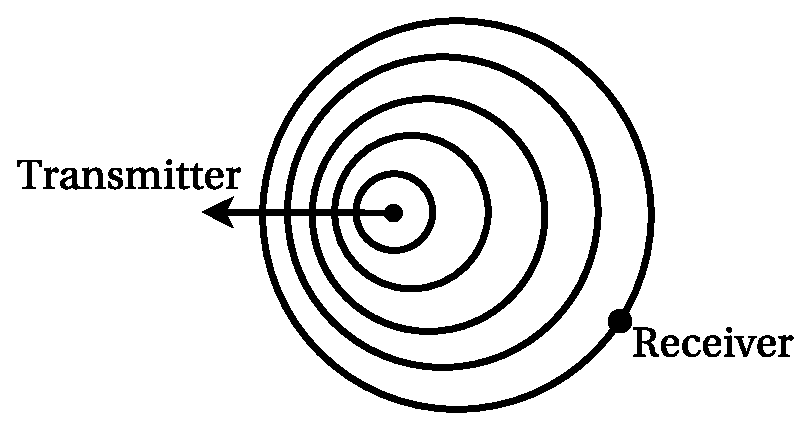
\includegraphics[width=0.45\textwidth,height=\textheight]{SensorsFigures/doppler.*}
\caption{Using the Doppler Effect to estimate velocity.}
\end{figure}

From physics we have the formulas for the change in sound. Assume the
speeds of source and the receiver relative to the medium are lower than
the velocity of waves in the medium.

Then the relationship between observed frequency \(f\) and emitted
frequency \(f_0\) is given by:

\[{\displaystyle f=\left({\frac {c\pm v_{\text{r}}}{c\pm v_{\text{s}}}}\right)f_{0}}\]

where

\begin{quote}
c is the propagation speed of waves in the medium;
\({\displaystyle v_{\text{r}}}\) is the speed of the receiver relative
to the medium, added to c if the receiver is moving towards the source,
subtracted if the receiver is moving away from the source;
\({\displaystyle v_{\text{s}}}\) is the speed of the source relative to
the medium, added to c if the source is moving away from the receiver,
subtracted if the source is moving towards the receiver.
\end{quote}

Note this relationship predicts that the frequency will decrease if
either source or receiver is moving away from the other.

\hypertarget{gyroscopes}{%
\subsection{Gyroscopes}\label{gyroscopes}}

The word pose is used for both position and orientation. Measurement of
orientation is done through several basic sensing approaches which we
discuss here.

A \texttt{gyroscope} is a heading sensor that gives a measure of
orientation with respect to a fixed frame. A standard gyro provides an
absolute measure of the heading for a mobile robot normally measured in
degrees off of some fixed heading. The classical mechanical gyroscope
uses a spinning body and the resulting rotational inertia. Optical gyros
can use phase shifts of intersecting beams of light to measure changes
in orientation. Rate gyros give a measure of angular speeds which is the
standard for low-cost MEMS systems. These are the most common units
found in mobile robots, UAVs, phones and other portable devices. These
gyros will return data in degrees per second (deg/s). Like
accelerometers, the MEMS units (microelectromechanical systems) are
packaged into 1, 2, 3 sensors to provide rotational rates about the
\(x\), \(y\) and \(z\) axes. Also like the accelerometer, the gyro can
have a digital or analog interface.

Drift can be a significant issue. The absolute direction can be lost
over a period of time depending on the sensor quality. This is an issue
that must be addressed for systems which run for long periods of time
without a recalibration.

\begin{quote}
Tuning fork MEMS gyroscope.
\end{quote}

\hypertarget{compass}{%
\subsection{Compass}\label{compass}}

The \texttt{compass} or \texttt{magnetometer} is one of the oldest
sensors in use dating back 4000 years. Early forms would take a small
piece of loadstone (natural magnetite) and suspend it from a silk thread
or place it on wood and float that in water. This magnetic rock would
orient along the Earth's field lines and could then be used for
navigation. Due to the liquid iron core, the Earth's field is
sufficiently strong to measure with portable devices. Although pole
reversals do occur, we have relatively stable pole locations for long
periods of time, so compass navigation has been a popular orientation
tool for thousands of years. This is an absolute measure of orientation
in contrast to the relative sensing we saw with the radial encoder.

There are multiple ways to measure a magnetic field. The traditional
methods are known as mechanical in that the force of the field lines
induces a torque and moves part of the sensor. Other approaches use the
Hall-Effect or Magnetoresistive sensors. The earth's magnetic field is
still relatively weak. Other magnetic sources such as inductors can
disturb and invalidate measurements. It is critical when building the
sensing system, the sensor is not placed near a motor, power supply or
any other device which can generate magnetic interference. Large amounts
of iron can alter the earth's field or even shield it. This prevents a
magnetic sensing in certain environments.

\hypertarget{magnetic-encoding}{%
\subsubsection{Magnetic encoding}\label{magnetic-encoding}}

It is possible to use \texttt{Hall-Effect} or other similar devices to
do encoding. Small Hall-Effect sensors with sub-degreee accuracy are
available. Placing a small ceramic magnet on the end of a shaft will
generate a rotating magnetic field which can be detected with the
Hall-Effect sensor. Figure \texttt{halleffect} shows how this is done.

\begin{quote}
Hall-Effect based shaft rotation sensor.
\end{quote}

\hypertarget{accelerometers-and-inertial-sensing}{%
\subsection{Accelerometers and Inertial
Sensing}\label{accelerometers-and-inertial-sensing}}

An \texttt{accelerometer} measures acceleration in a particular
direction. The standard units on acceleration are meters per seconds
squared (\(m/s^2\)). The sensor is normally a MEMS unit which are often
packaged together using two or three sensor units pointed in orthogonal
directions. This can provide acceleration information along each of the
coordinate axes. Common constructions use two plates with one moveable
and attached to a mass, and the other fixed. Acceleration will cause the
plate to move and change the capacitance. This change can be measured
and related to the acceleration. Output may be a voltage level in which
the sensor is known as an analog sensor or the output can be through a
digital interface, such as I\(^2\)c making it a digital sensor.

\begin{quote}
Simple accelerometer structure.
\end{quote}

A simple application of an accelerometer is an \texttt{inclineometer} or
tilt sensor. These sensors can have a great deal of noise and extracting
a good signal can be very challenging. Note that it is temping to think
that this device can provide position information. After all, we learn
in calculus that if we integrate acceleration twice, we obtain position.
The problem is the noise. Even though integration is numerically a
smoothing process which can reduce noise by averaging it out, over time
small errors build and position accuracy is poor. In practice, using an
accelerometer does not provide adequate position or velocity estimates.

\hypertarget{inertial-measurement-unit-imu}{%
\subsection{Inertial Measurement Unit
(IMU)}\label{inertial-measurement-unit-imu}}

An \texttt{Inertial\ Measurement\ Unit} or \texttt{IMU} packages
accelerometers, gyroscopes and possibly a compass together into a single
unit. A 6DOF (degrees of freedom) IMU will have a three axis
accelerometer and three axis gyroscope. A 9DOF IMU will have the three
axis accelerometer, three axis gyroscope and a 3 axis magnetometer.
These devices normally provide a digital interface such as USB and
return text strings of data at some Hz. IMUs are used as the basis for
AHRS: Attitude and Heading Reference System.

\hypertarget{attitude-and-heading-reference-system-ahrs}{%
\subsection{Attitude and Heading Reference System
(AHRS)}\label{attitude-and-heading-reference-system-ahrs}}

\texttt{AHRS} consist of accelerometers, gyroscopes and magnetometers on
all three axes. So, AHRS includes an IMU. In addition to the IMU, the
AHRS has the algorithms to provide attitude and heading information as
well as the required hardware for the computation. These algorithms
include sensor fusion codes which take data from multiple sources and
"fuse" them into a hopefully more accurate picture of the measured
quantity. A popular estimator known as the Kalman Filter is used to do
the fusion and state estimation. A variant of AHRS is an Inertial
Navigation System (INS). The difference is that INS estimates attitude,
position and velocity.

\textbf{Footnotes}
